\chapter{Создание базы данных}
\section{Работа по методическим указаниям}
Создадим базу данных \texttt{forum}, которая хранит в себе сведения о пользователях форумах и размещенных ими темах.

Помимо суперпользователя root, был создан пользователь denilai, под которым производятся все манипуляции с данными.

Создадим базу данных \texttt{forum} с помощью команды \texttt{CREATE DATABASE forum;}


Создадим таблицу \texttt{users} (см. Рисунок \ref{fig:create-users}):

% TODO: \usepackage{graphicx} required
\begin{figure}[h!]
	\centering
	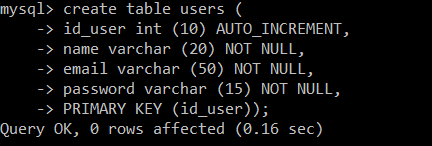
\includegraphics[width=0.7\linewidth]{create-users}
	\caption{Создание базы данных users}
	\label{fig:create-users}
\end{figure}

%\begin{lstlisting}
%create table users (
%	id_user INT (10) AUTO_INCREMENT,
%	name varchar(20) NOT NULL,
%	email varchar(50) NOT NULL,
%	password varchar(15) NOT NULL,
%	PRIMARY KEY (id_user)
%);
%\end{lstlisting}

Создадим таблицу \texttt{topics} (см. Рисунок \ref{fig:create-topics}):

% TODO: \usepackage{graphicx} required
\begin{figure}[h!]
	\centering
	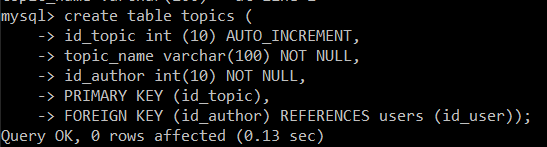
\includegraphics[width=0.7\linewidth]{create-topics}
	\caption{Создание базы данных topics}
	\label{fig:create-topics}
\end{figure}

%\begin{lstlisting}
%create table topics (
%	id_topic INT (10) AUTO_INCREMENT,
%	topic_name varchar(100) NOT NULL,
%	id_author INT (10) NOT NULL,
%	PRIMARY KEY (id_topic),
%	FOREIGN KEY (id_author) REFERENCES users (id_user)
%);
%\end{lstlisting}
Создадим таблицу \texttt{posts} (см. Рисунок \ref{fig:create-posts}):

\begin{figure}[h!]
	\centering
	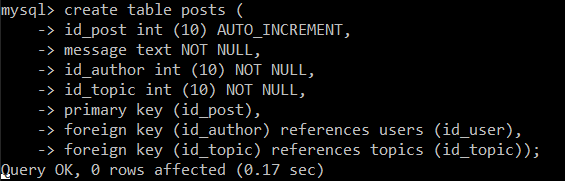
\includegraphics[width=0.7\linewidth]{create-posts}
	\caption{Создание базы данных posts}
	\label{fig:create-posts}
\end{figure}

После создания таблиц, заполним их данными о пользователях форума, о темах и размещенных публикациях. Выполним операцию выборки данных без условия, чтобы увидеть все записи, занесенные в таблицы с помощью команды \texttt{SELECT * FROM <table-name>} (см. Рисунок \ref{fig:select-from-all}). 

% TODO: \usepackage{graphicx} required
\begin{figure}[h!]
	\centering
	\includegraphics[width=0.8\linewidth]{select-from-all}
	\caption{Операция выборки из всех таблиц }
	\label{fig:select-from-all}
\end{figure}

Выполним запрос \texttt{SELECT mesage, topic\_name FROM posts p JOIN topics t ON t.id\_author = p.id\_author; } для объединения данных из таблиц \texttt{topics} и \texttt{posts} по ключу id\_author и получения полной информации о сообщении и названию темы, в которой оно было размещено (см. Рисунок \ref{fig:join-post-author}).

% TODO: \usepackage{graphicx} required
\begin{figure}[ht]
	\centering
	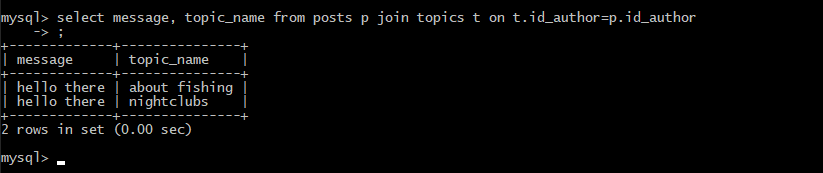
\includegraphics[width=0.8\linewidth]{join-post-author}
	\caption{Запрос объединения}
	\label{fig:join-post-author}
\end{figure}

Выполним запрос выборки данных, явно указав поля отношения. Для этого перечислим имена полей через запятую после зарезервированного слова \texttt{SELECT} (см. Рисунок \ref{fig:field-select}).

% TODO: \usepackage{graphicx} required
\begin{figure}[h!]
	\centering
	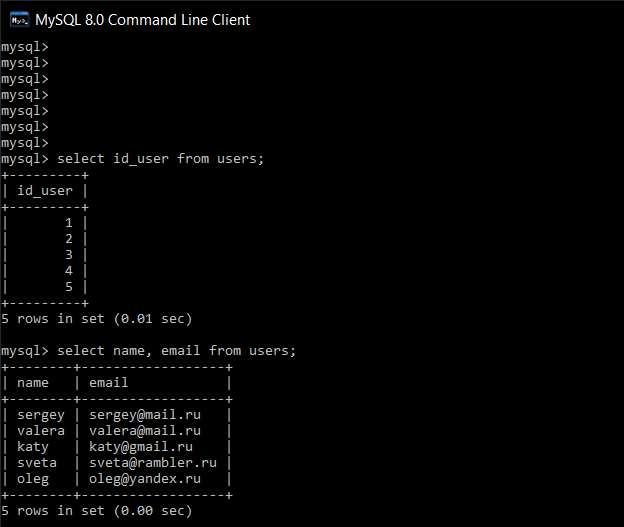
\includegraphics[width=0.5\linewidth]{field-select}
	\caption{Операция выборки с указанием полей}
	\label{fig:field-select}
\end{figure}


Выполним более сложные запросы выборки, отсортировав записи в таблице \texttt{topics} по убыванию значения поля \texttt{topic\_name} и \texttt{id\_author}, а также опишем условие сравнения значения поля \texttt{id\_author} в сецкции \texttt{WHERE}(см. Рисунок \ref{fig:order-where-forum}). 

% TODO: \usepackage{graphicx} required
\begin{figure}[h!]
	\centering
	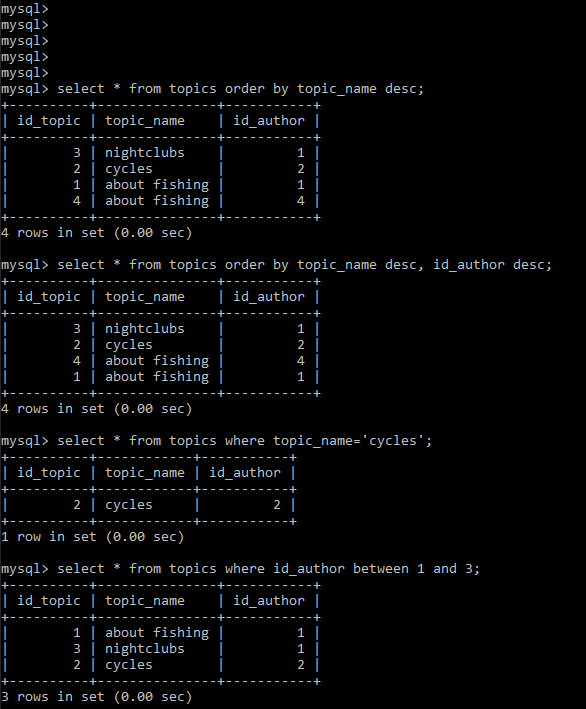
\includegraphics[width=0.5\linewidth]{order-where-forum}
	\caption{Сложные запросы выборки с сортировкой и условием}
	\label{fig:order-where-forum}
\end{figure}

Выполним операции по модификации таблицы --- добавим в таблицу \texttt{users} поле \texttt{country} типа \texttt{varchar (20)} со значением по умолчанию "Russia", а также добавим в эту же таблицу поле \texttt{age int(10)} со значением по умолчанию 19. 

Выведем все записи из таблицы \texttt{users}, обнаружим, что столбцы были вставлены успешно (см. Рисунок \ref{fig:alter-add-forum}).

% TODO: \usepackage{graphicx} required
\begin{figure}[h!]
	\centering
	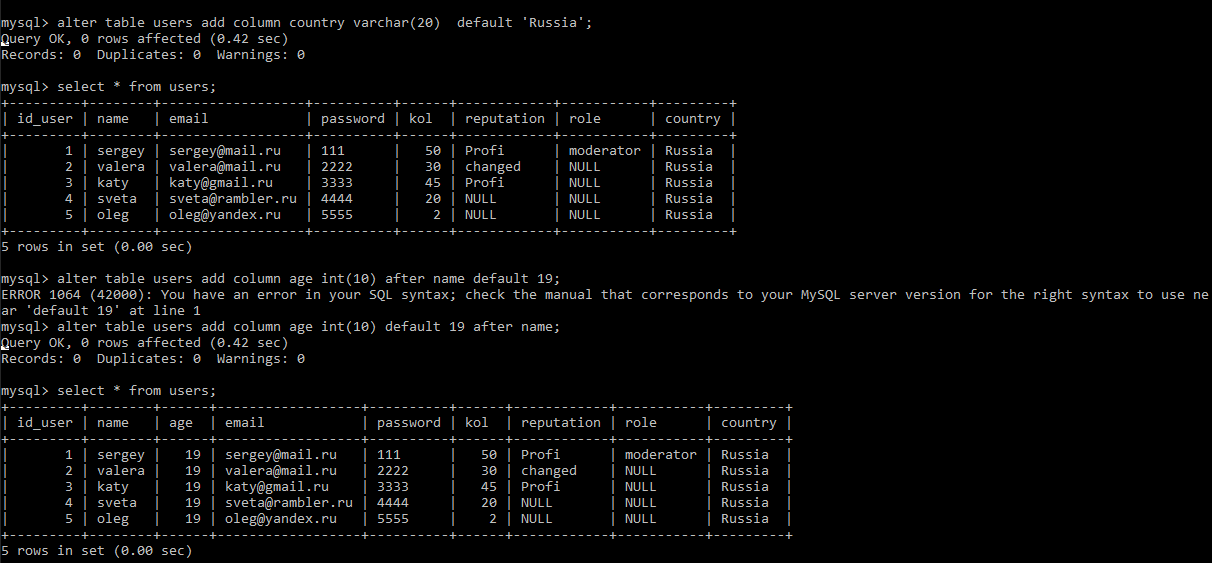
\includegraphics[width=0.9\linewidth]{alter-add-forum}
	\caption{Добавление полей в таблицу \texttt{users}}
	\label{fig:alter-add-forum}
\end{figure}

В ходе данной практической работы были рассмотрены операторы DDL и DML диалекта MySQL. С помощью данных операторов была создана база учебная база данных \texttt{forum}, содержащая о пользователях форумах и размещенных ими темах.

\section{Индивидуальное задание}

Продолжим работу над созданием модели данных велосипедного предприятия. Создадим базу данных \texttt{cycle}, сущностями  которой будут таблицы, описания которых были проработаны в прошлых практических работах. 

Описание проектируемых отношений базы данных \texttt{cycle} приведены в таблицах \ref{tab:bar}--\ref{tab:log}.

%(\textbf{Bar})
\begin{table}[h!] 
	\centering
	\caption{Описание таблицы Bar}
	\begin{tabular}{|l|l|}
		\hline \textbf{Имя} & \textbf{Тип} \\
		\hline
		Width & INTEGER NOT NULL \\ \hline
		Diameter & INTEGER NOT NULL \\ \hline
		BarID & INTEGER NOT NULL AUTO\_INCREMENT \\ \hline
		Color & VARCHAR(20) NULL DEFAULT 'black' \\ \hline
	\end{tabular}
	\label{tab:bar}
\end{table}

%(\textbf{Brake})
\begin{table}[h!] 
	\centering
	\caption{Описание таблицы Brake}
	\begin{tabular}{|l|l|}
		\hline \textbf{Имя} & \textbf{Тип} \\
		\hline
		BrakeID &       INT NOT NULL AUTO\_INCREMENT \\ \hline
		ComponentID &   INTEGER NULL \\ \hline
	\end{tabular}
	\label{tab:brake}
\end{table}


%(\textbf{Component})

\begin{table}[h!] 
	\centering
	\caption{Описание таблицы Component}
	\begin{tabular}{|l|l|}
		\hline \textbf{Имя} & \textbf{Тип} \\
		\hline
		ComponentID &   INTEGER NOT NULL AUTO\_INCREMENT \\ \hline
		Brand & VARCHAR(20) NOT NULL \\ \hline
		ManufacturerCountry &  VARCHAR(20) NOT NULL \\ \hline
		PriceCent & INTEGER NOT NULL \\ \hline
		Model & VARCHAR(20) NOT NULL \\ \hline
		ComponentTypeID &  INTEGER NOT NULL \\ \hline
		WeightGramm &   INTEGER NOT NULL \\ \hline
	\end{tabular}
	\label{tab:component}
\end{table}

%(\textbf{ComponentType}) 
\begin{table}[h!] 
	\centering
	\caption{Описание таблицы ComponentType}
	\begin{tabular}{|l|l|}
		\hline \textbf{Имя} & \textbf{Тип} \\
		\hline
		ComponentTypeID &  INTEGER NOT NULL AUTO\_INCREMENT \\ \hline
		Name & VARCHAR(20) \\ \hline
	\end{tabular}
	\label{tab:componenttype}
\end{table}


%(\textbf{CycleType})

\begin{table}[h!] 
	\centering
	\caption{Описание таблицы CycleType}
	\begin{tabular}{|l|l|}
		\hline \textbf{Имя} & \textbf{Тип} \\
		\hline
		CycleTypeID &   INTEGER NOT NULL AUTO\_INCREMENT \\ \hline
		Name &  VARCHAR(20) NOT NULL \\ \hline
	\end{tabular}
	\label{tab:cycletype}
\end{table}

\begin{table}[h!] 
	\centering
	\caption{Описание таблицы FctCycleBuild}
	\begin{tabular}{|l|l|}
		\hline \textbf{Имя} & \textbf{Тип} \\
		\hline
		SetupID &       INTEGER NOT NULL \\ \hline
		Datetime &      DATE NOT NULL \\ \hline
		Stage & INTEGER NOT NULL \\ \hline
		Workshop &      varchar(20) NOT NULL DEFAULT 'main' \\ \hline
		Master &        VARCHAR(20) NOT NULL \\ \hline
		Status &        VARCHAR(20) NOT NULL \\ \hline
		Comment &       VARCHAR(20) NOT NULL \\ \hline
	\end{tabular}
	\label{}
\end{table}

%(\textbf{Fork})

\begin{table}[h!] 
	\centering
	\caption{Описание таблицы Fork}
	\begin{tabular}{|l|l|}
		\hline \textbf{Имя} & \textbf{Тип} \\
		\hline
		ForkID &  INTEGER NOT NULL AUTO\_INCREMENT \\ \hline
		Color & VARCHAR(20) NULL DEFAULT 'black' \\ \hline
		ComponentID &  INTEGER NULL \\ \hline
	\end{tabular}
	\label{ta:fork}
\end{table}


%(\textbf{Frame})

\begin{table}[h!] 
	\centering
	\caption{Описание таблицы Frame}
	\begin{tabular}{|l|l|}
		\hline \textbf{Имя} & \textbf{Тип} \\
		\hline
		FrameID &  INTEGER NOT NULL AUTO\_INCREMENT \\ \hline
		Color & VARCHAR(20) NULL DEFAULT 'black' \\ \hline
	\end{tabular}
	\label{tab:frame}
\end{table}


%(\textbf{FrameInfo})

\begin{table}[h!] 
	\centering
	\caption{Описание таблицы FrameInfo}
	\begin{tabular}{|l|l|}
		\hline \textbf{Имя} & \textbf{Тип} \\
		\hline
		FrameID &       INTEGER NOT NULL \\ \hline
		Size & INTEGER NOT NULL \\ \hline
		Stack & INTEGER NOT NULL \\ \hline
		Reach & INTEGER NOT NULL \\ \hline
	\end{tabular}
	\label{tab:frameinfo}
\end{table}


%(\textbf{Frameset})

\begin{table}[h!] 
	\centering
	\caption{Описание таблицы Frameset}
	\begin{tabular}{|l|l|}
		\hline \textbf{Имя} & \textbf{Тип} \\
		\hline
		FrameSizeID &   INTEGER NOT NULL AUTO\_INCREMENT \\ \hline
		ForkID &        INTEGER NOT NULL \\ \hline
		FramesetID &    INTEGER NOT NULL \\ \hline
		ComponentID &   INTEGER NOT NULL \\ \hline
	\end{tabular}
	\label{tab:frameset}
\end{table}


%(\textbf{FrameSize})

\begin{table}[h!] 
	\centering
	\caption{Описание таблицы FrameSize}
	\begin{tabular}{|l|l|}
		\hline \textbf{Имя} & \textbf{Тип} \\
		\hline
		FrameID &       INTEGER NOT NULL \\ \hline
		Size &  INTEGER NOT NULL \\ \hline
		FrameSizeID &   INTEGER NOT NULL AUTO\_INCREMENT \\ \hline
		ComponentID &   INTEGER NOT NULL \\ \hline
	\end{tabular}
	\label{tab:framesize}
\end{table}


%(%(\textbf{Groupset}))

\begin{table}[h!] 
	\centering
	\caption{Описание таблицы Groupset}
	\begin{tabular}{|l|l|}
		\hline \textbf{Имя} & \textbf{Тип} \\
		\hline
		Ratio & INTEGER NOT NULL \\ \hline
		BrakeID &       CHAR(18) NOT NULL \\ \hline
		GroupsetID &    INTEGER NOT NULL AUTO\_INCREMENT \\ \hline
		Color & VARCHAR(20) NOT NULL \\ \hline
		ComponentID &   INTEGER NOT NULL \\ \hline
	\end{tabular}
	\label{tab:groupset}
\end{table}


%(\textbf{Setup})

\begin{table}[h!] 
	\centering
	\caption{Описание таблицы Setup}
	\begin{tabular}{|l|l|}
		\hline \textbf{Имя} & \textbf{Тип} \\
		\hline
		GroupsetID &    INTEGER NOT NULL \\ \hline
		WheelsetID &    INTEGER NOT NULL \\ \hline
		FramesetID &    INTEGER NOT NULL \\ \hline
		BarID & INTEGER NOT NULL \\ \hline
		CycleTypeID &   INTEGER NOT NULL \\ \hline
		SetupID &       INTEGER NOT NULL AUTO\_INCREMENT \\ \hline
	\end{tabular}
	\label{tab:setup}
\end{table}


%(\textbf{Wheelset})

\begin{table}[h!] 
	\centering
	\caption{Описание таблицы Wheelset}
	\begin{tabular}{|l|l|}
		\hline \textbf{Имя} & \textbf{Тип} \\
		\hline
		DiametrInch &   INTEGER NOT NULL \\ \hline
		Width & INTEGER NOT NULL \\ \hline
		SpokesCount &   INTEGER NULL \\ \hline
		WheelsetID &    INTEGER NOT NULL AUTO\_INCREMENT \\ \hline
		Color & VARCHAR(20) NOT NULL \\ \hline
		ComponentID &   INTEGER NOT NULL \\ \hline
	\end{tabular}
	\label{tab:wheelset}
\end{table}

\begin{table}[h!] 
	\centering
	\caption{Описание таблицы Log}
	\begin{tabular}{|l|l|}
		\hline \textbf{Имя} & \textbf{Тип} \\
		\hline
		ID &   INTEGER NOT NULL AUTO\_INCREMENT \\ \hline
		msg & VARCHAR{100} NOT NULL \\ \hline
		row\_id & INTEGER NOT NULL \\ \hline
	\end{tabular}
	\label{tab:log}
\end{table}



\newpage\hfill\newpage\hfill\newpage

\subsection{Использование MySQL CLI Client}

Создадим данные таблицы с помощью MySQL CLI Client~---~клиента, предоставляющего доступ к СУБД через интерфейс командой строки, использовав ключевое слово \texttt{CREATE TABLE}. После создания таблиц выполним команду \texttt{SHOW TABLES}, выбрав базу данных \texttt{cycle} (см. Рисунок \ref{fig:show-tables-cycle}).

% TODO: \usepackage{graphicx} required
\begin{figure}[h!]
	\centering
	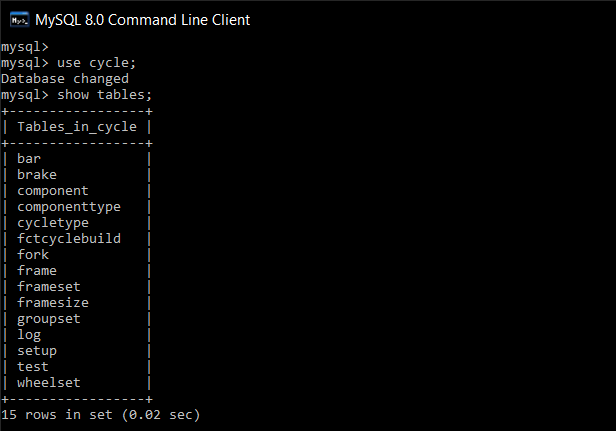
\includegraphics[width=0.5\linewidth]{show-tables-cycle}
	\caption{таблицы базы данных \texttt{cycle}}
	\label{fig:show-tables-cycle}
\end{figure}
Выведем записи из таблицы \texttt{Component} (см. Рисунок \ref{fig:select-components}).

% TODO: \usepackage{graphicx} required
\begin{figure}[h!]
	\centering
	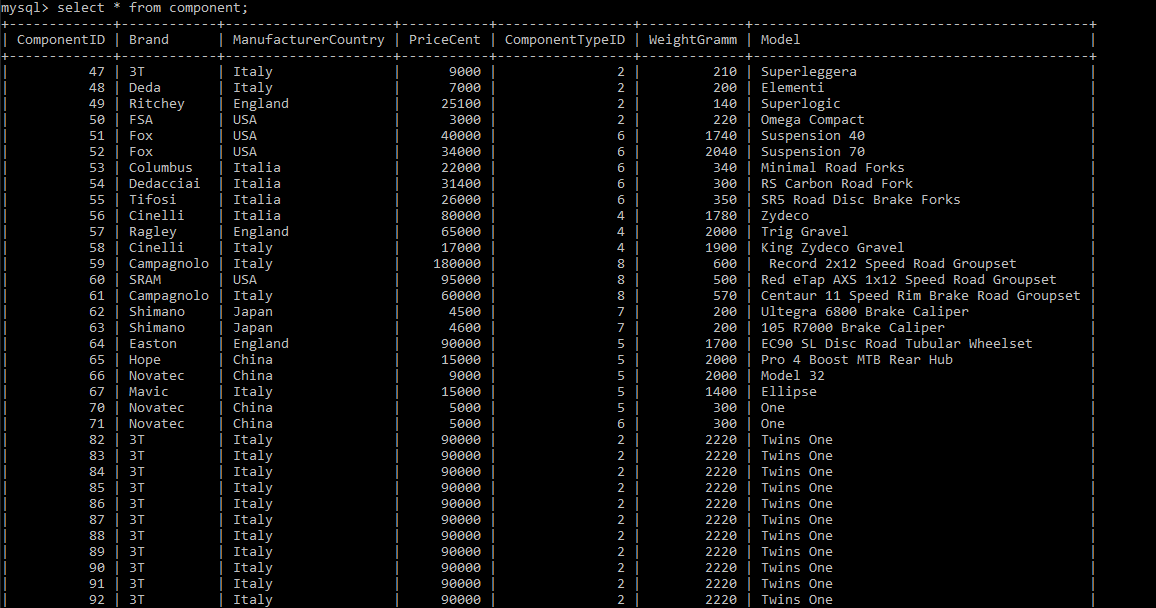
\includegraphics[width=\linewidth]{select-components}
	\caption{Вывод записей из таблицы Components}
	\label{fig:select-components}
\end{figure}

Выполним более сложные запросы выборки --- объединим таблицы с помощью оператора \texttt{INNER JOIN} \texttt{Component} и \texttt{fork} по полю \linebreak \texttt{component\_id}, а также воспользуемся функцией \texttt{ROW\_NUMBER()} в сочетании с оконной функцией \texttt{OVER()}, пронумеровав компоненты из таблицы \texttt{Fork} одного цвета по возрастанию значения поля \texttt{color} (см. Рисунок \ref{fig:join-window-cycle}).

% TODO: \usepackage{graphicx} required
\begin{figure}[h!]
	\centering
	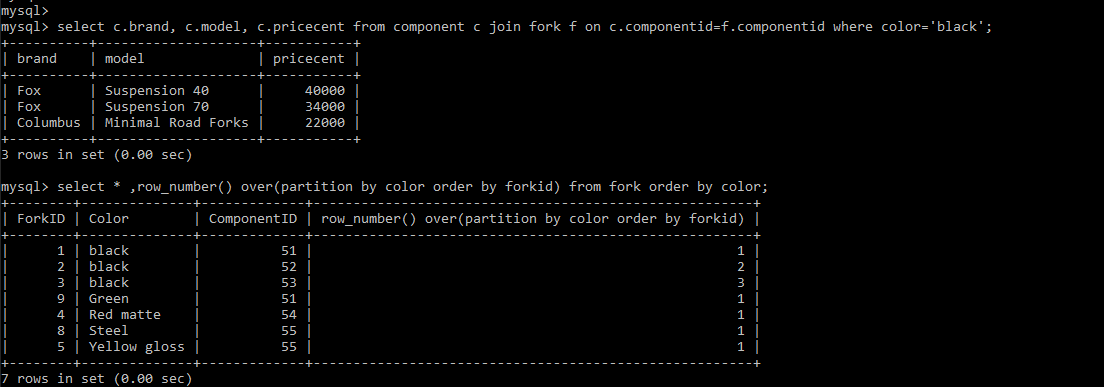
\includegraphics[width=\linewidth]{join-window-cycle}
	\caption{Сложные запросы выборки. База данных cycle}
	\label{fig:join-window-cycle}
\end{figure}


Создадим триггеры \texttt{delete\_component} и  \texttt{add\_component} на добавление и удаление записи в таблице \texttt{Component}. При срабатываении данного триггера, будет добавляться запись в таблицу log, информирующая о совершении манипуляций с данными (см. Листинг \ref{list:trigger}).
%\newpage
Приведем объявление данного триггера на диалекте MySQL:
\lstset{
	language=sql
}
\begin{lstlisting}[caption=Триггер, label={list:trigger}]
DELIMITER $$
drop trigger delete_component; $$

create trigger `delete_component` after delete on component
for each row begin
insert into log (msg, row_id) values (concat('delete component ',old.Brand,' ', old.Model), old.ComponentID);
end; $$

create trigger `add_component` after insert on component
for each row begin
insert into log (msg, row_id) values (concat('insert component ',new.Brand,' ', new.Model), new.ComponentID);
end; $$
DELIMITER $$
\end{lstlisting}

\subsection{Использование MySQL Workbench}

Выполним операции по изменению и просмотру данных, занесенных в базу данных \texttt{cycle}, с помощью инструмента для визуального проектирования баз данных MySQL Workbench.

Для этого подключимся к локально развернутому на машине MySQL Server, указав порт, имя пользователя и пароль. После этого мы получим доступ к пользовательскому интерфейсу программы, представляющему собой две области~---~область выполнения запросов и область отображения результатов (см. Рисунок \ref{fig:workbrench-interface}).

\begin{figure}[h!]
	\centering
	\includegraphics[width=\linewidth]{figures/web-clent/workbrench-interface}
	\caption{Интерфейс MySQL Workbench}
	\label{fig:workbrench-interface}
\end{figure}

Создадим временную таблицу, в котором объединим сведения о компонентах (см. Рисунок \ref{fig:workbrench-components}).
\begin{figure}[h!]
	\centering
	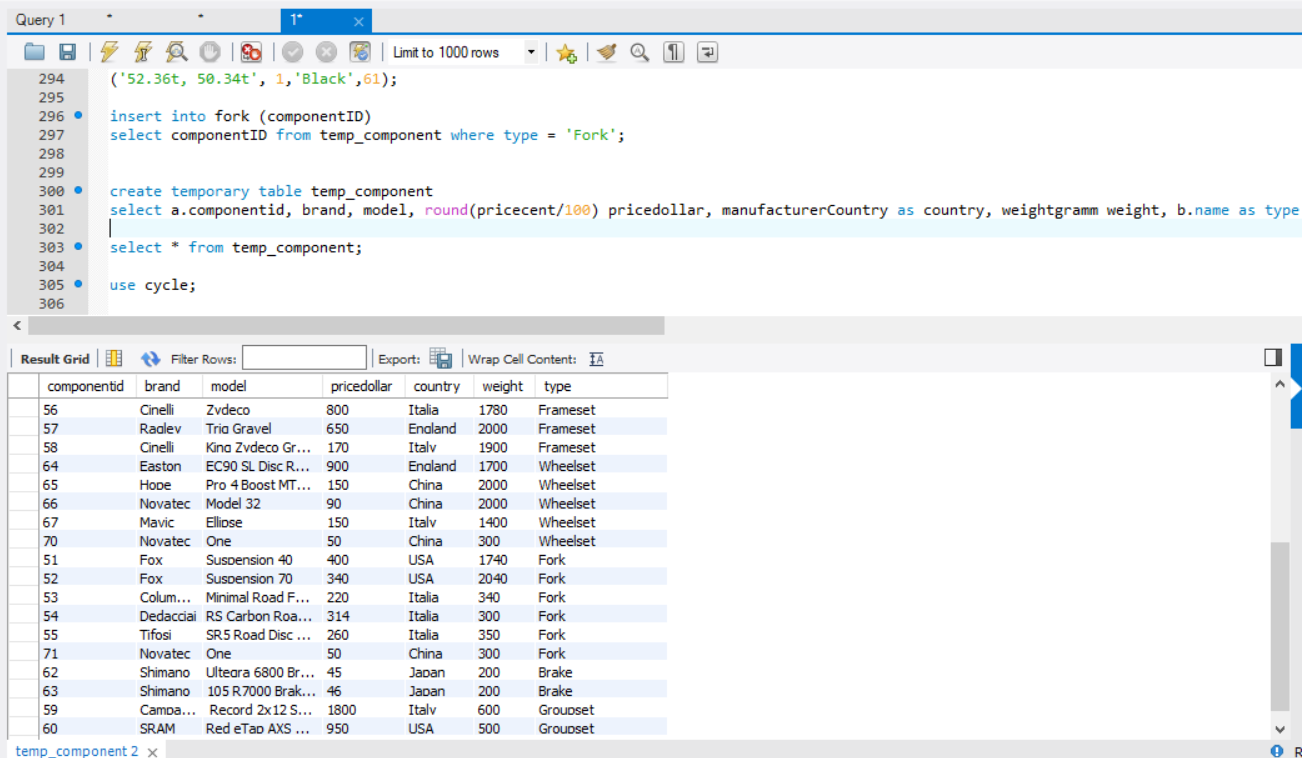
\includegraphics[width=1\linewidth]{figures/web-clent/workbrench-components}
	\caption{Просмотр временной таблицы компонентов}
	\label{fig:workbrench-components}
\end{figure}

Выполним еще один запрос~---~ограничим вывод только компонентами типа <<Fork>> (см. Рисунок \ref{fig:workbrench-forks}).

\begin{figure}[h!]
	\centering
	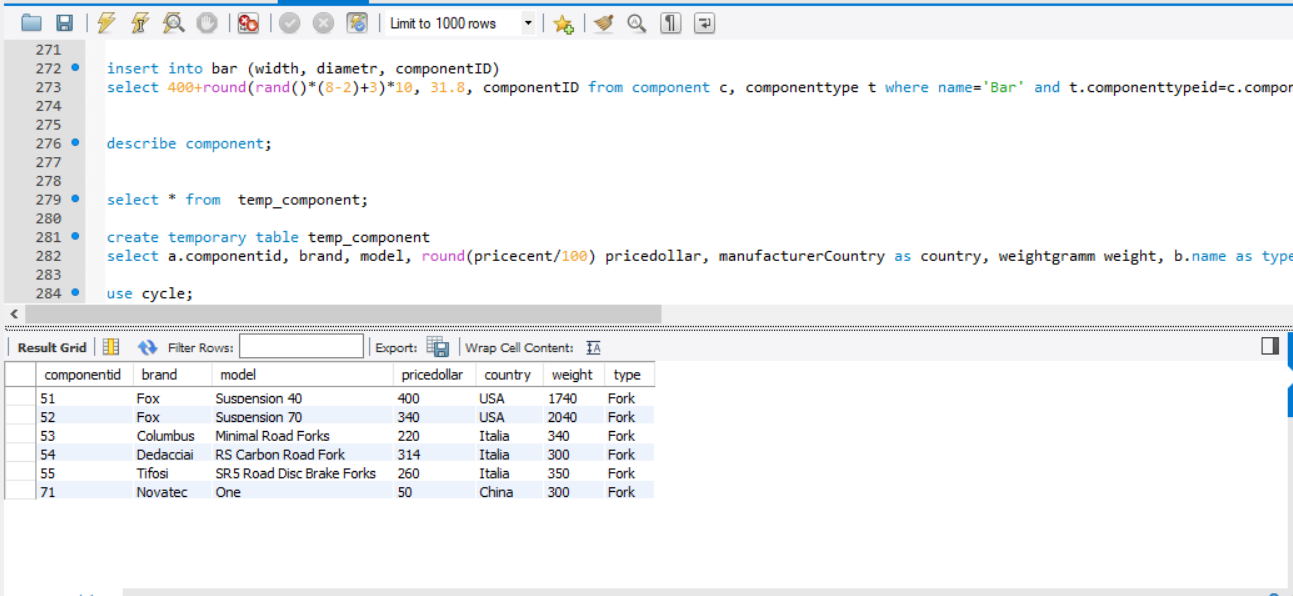
\includegraphics[width=1\linewidth]{figures/web-clent/workbrench-forks}
	\caption{Просмотр временной таблицы компонентов. Компоненты <<Fork>>}
	\label{fig:workbrench-forks}
\end{figure}

Данный визуальный инструмент позволяет удобно организовать работу с базой данных, сохранять SQL--скрипты, параметры подключения и настройки.